\chapter{Modelling}
	This chapter summarises the problem and assumptions taken considering the pipeline following problem.
	A controller will be derived for tracking and maneuvering of the AUV vehicle. A Kalman filter
	will be derived for the smoothing of measurements and predictions of the pipeline. A guidance algorithm will
	be presented and discussed. The behaviour of the system will be treated in the last sections of this chapter,
	where a proposed flow of the decision process will be presented.


\section{Problem Outline}
\label{chap2:problem}
	To solve the pipeline following problem it is important to have a clear formulation of the problem.
	This is a path following problem, since the pipeline can be represented as a continuous path in
	space. The geometric convergence to the path is the primary objective, and any dynamical
	constraints along the path, i.e velocity constraints, are considered secondary to the goal of
	geometric convergence. When there are dynamic constraints the problem is a Trajectory Tracking
	Problem. If only geometric convergence are considered the problem is called a Path Following Problem, 
	as stated in the definitions in Chapter~\ref{chap1-guidance-alg}

	In this report the pipeline will be formulated as a two dimensional path. This because the pipeline
	are laid on the sea bottom, and are assumed to follow the bottom signature. Then the path following
	is reduced to a two dimensional problem. The \textit{heave} state can be decoupled from the guidance 
	system design. The depth controller then needs to keep a constant height above the sea bottom.
	This ignores the possibility of free spanning pipelines.

	In order to limit the problem and ease the implementation, the pipeline are assumed to be a straight
	or nearly straight, piece-wise continuous line segment. The pipeline can only change direction at defined
	places called junctions. This reduces the application of this guidance system to only concider long,
	continuous stretches of piplines. 

	An AUV carrying out a pipeline inspection mission in most cases,  renders the low speed assumption valid.
	The \hugin AUV are designed for speeds from 0-3 m/s. The inspection speed assumed in the
	rest of the report are around 1 m/s. This are relatively low speed, and the quadratic terms in the
	Coriolis/centripetal or Damping matices can be neglected. 

	\begin{figure}[hbtp]
		\centering
		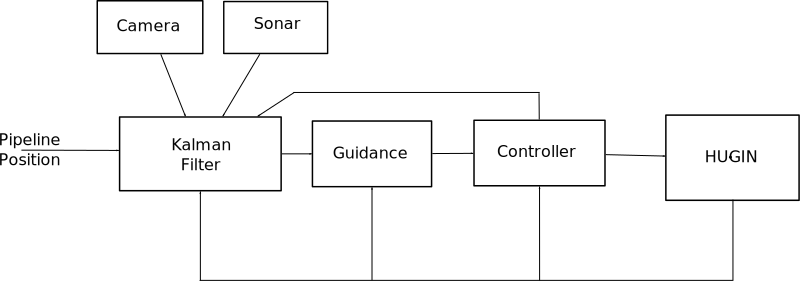
\includegraphics[width=0.9\textwidth]{pics/blockdiagram}
		\caption{Block diagram the path following controller}
		\label{fig:ch2-blockdiagram}
	\end{figure}
	As outlined in Figure \ref{fig:ch2-blockdiagram} the building blocks of the pipeline following
	control system are the cruising controller, guidance system and the filter
	which fuses the known data about the pipeline and the measured pipeline data. To recreate the 
	pipeline coordinates in three dimensions the distance to the sea bottom is measured by a sonar. The
	filter uses prior knowledge about the pipeline to-be-followed, which are assumed to be inaccurate. 
	The filter uses this information together with the altitude information and camera output to estimate the
	position of the pipeline. If the pipeline should be lost at any time the filter will try to predict
	where the pipeline are, and still give input to the guidance block.
	
	The system should be able to handle buried sections of the pipeline. The camera will not be able to
	sense the pipeline during the buried stretch and other sensors should be included. A bottom
	penetrating sonar might be used for this purpose, or a magnetic pipe tracker. These sensors are able
	to sense the pipeline even if buried up to 3 meters. \cite{PhD_lecture} These sensors will better the
	AUVs chances to regain track after the buried stretch, than if it were to relay just on dead
	reckoning from the predicted pipeline information alone.

\section{Pipeline Representation}
	The representation of the pipeline is important because it is used in the Kalman filter to predict
	where the pipeline is going. The pipeline is parametrised by $\varpi \in \mathbb{R}$ to get a
	continuous and smooth pipeline.

	In this report the pipeline are parametrised as:
	\begin{equation}
		P_w(\varpi) = \left [ \begin{array}{c}
					\varpi \\
					k_y \varpi \\
					z(\eta)
				\end{array} \right ] \quad \varpi \in (0, \infty)
	\end{equation}
	where $k_y$ are constant and $z(\eta)$ is some function described by the sea bottom and are assumed
	known. This represents the straight line as the pipeline are assumed to be.
	
	


\section{Kalman Filter}
	The Kalman filters purpose is to smooth the camera output and predict forward where the pipeline will
	be in the future, to supply a better heading reference for the guidance controller.

	The position of the pipeline are given some uncertainty because the pipeline may have moved after it
	was laid, or the navigation system of the AUV might be erroneous and give wrong position. This gives the
	following model of the pipeline:
	\begin{equation}
		P_w(\varpi) = \left [ \begin{array}{c}
					\varpi \\
					k_y \varpi \\
					z(\eta)
				\end{array} \right ] + \mathbf{B}\delta
	\end{equation}
	The function $\delta$ are a slowly varying disturbance which can be modeled as a \textit{1st order Markov
	Process}, and $\mathbf{B}$ is some 2x3 matrix.
	\begin{equation}
		\dot{\delta} = -\mathbf{T} \delta +  w
	\end{equation}
	where $w \in \mathbb{R}^2$, are a zero mean, unity variance, white noise process, which describes the
	error in the position. The matrix $\mathbf{T}$ specifies how the error evolves. Because the error are
	slowly varying the eigenvalues of $\mathbf{T}$ should be chosen large. Time differentiating
	the position estimate gives
	\begin{equation}
		\dot{P_w}(\varpi) =  \left [ \begin{array}{c}
						\dot{\varpi} \\
						k_y \dot{\varpi} \\
						\dot{z}(\eta)
					\end{array} \right ] + \dot{\delta}
	\end{equation}
	By setting $\varpi = N(t)$, i.e the North position and completely disregarding the depth coordinate.
	gives the following
	\begin{equation}
		\dot{P_w'} = \left [ \begin{array}{c}
					n \\
					k_y n 
				\end{array} \right ] + \dot{\delta}
	\end{equation}
	where $n$ is the rate that the AUV are moving towards north.
	Choosing the state vector and input as:
	\begin{equation}
		x = [ P_w'^T \quad \delta^T]^T \quad \Rightarrow  \quad \dot{x} = [\dot{P_w'^T} \quad
		\dot{\delta^T}]^T \quad  u = n
	\end{equation}
	This calls for the following state space representation 
	\begin{equation}
		\dot{x} = \left [ \begin{array}{cc}
					0 & -T \\
					0 & -T
				\end{array} \right] x + \left [ \begin{array}{c}
								1 \\
								k_y\\
								0 \\
								0
								\end{array} \right] u +
				\left [ \begin{array}{c}
						\mathbf{0}_{2x2} \\
						\mathbf{I}_{2x2} 
					\end{array} \right] w
	\end{equation}
	This state space are non-minimal because of the linear dependent rows and could be eliminated, but it makes no
	difference with regard to the estimation.

	The measurement model are more complex. In order to compare the measurement from the camera with the
	state space model, the perspective equations from Section \ref{ch1-cameramodel} are needed. By using
	Equations \eqref{eq:ch1-P_c} and \eqref{eq:ch1-perspective}, we can transform the point from world
	coordinates, i.e. coordinates decomposed in the NED-frame, to image coordinates. We want $y = P_i$
	\begin{equation*}
		y = P_i = \mathbf{H} P_c = \mathbf{H R}^T ( P_w - O(t))
	\end{equation*}
	$O(t)$ is the origin of the camera frame and is equal to the position vector $\eta' = [N(t),
	E(t)]^T$ of the AUV in the NED frame. By including the position vector in the input to the filter and using 
	$P_w = \mathbf{C} x$, the measurement model are concluded.
	\begin{equation}
		\label{eq:ch2-measurement}
		y = \mathbf{H R}^T \mathbf{C} x - \mathbf{H R}^T  O(t) = \mathbf{C}'x + \mathbf{D} u
	\end{equation}
	where $\mathbf{C'}$ and $\mathbf{D}$ are appropriate matrices for selecting the right states.
$\mathbf{R}$
	are the Rotation Matrix from World coordinates to Camera coordinates. This gives the following model
	for the Kalman filter
	\begin{align}
		x &= \mathbf{A} x + \mathbf{B} u + \mathbf{E} w\\
		y &= \mathbf{C}'x + \mathbf{D} u + v\\
		\mathbf{A} &= \left [ \begin{matrix}
					0 & 0 & -T_1 & 0 \\
					0 & 0 & 0 & -T_2 \\
					0 & 0 & -T_1 & 0 \\
					0 & 0 & 0 & -T_2 
					\end{matrix} \right] \quad \mathbf{B} = \left[ \begin{matrix}
										1 & 0 & 0 \\
										k_y & 0 & 0\\
										0   & 0 & 0 \\
										0 & 0 & 0
										\end{matrix} \right]\\
		\mathbf{E} &= \left [ \begin{matrix}
					0 & 0 \\
					0 & 0 \\
					1 & 0 \\
					0 & 1
					\end{matrix} \right] \quad \mathbf{C}' = \left [ \begin{matrix}
						\frac{f}{z_c} \cos{\psi} &\frac{f}{z_c} \sin{\psi} & 0 & 0 \\
						-\frac{f}{z_c} \sin{\psi}& \frac{f}{z_c} \cos{\psi} & 0 & 0 
								\end{matrix} \right] \\
		\mathbf{D} &= \left [ \begin{matrix}
					0 & -\frac{f}{z_c} \cos{\psi} & -\frac{f}{z_c} \sin{\psi} \\
					0 & \frac{f}{z_c} \sin{\psi} & -\frac{f}{z_c} \cos{\psi}
					\end{matrix} \right]
	\end{align}
	$w, v$ are a vectors of unity white noise and have covariance $E(ww^T) = \mathbf{Q}$ and $E(vv^T) =
	\mathbf{W}$. The filter should be run at the same frequency as the guidance system to provide output
	for the guidance system. The prediction will be updated whenever possible, which means when the
	pipeline are visible in the camera, after the image processing are finished.

	Because of the relatively high frequency of the filter the parameters in the measurement model
	regarding heading and depth, i.e. $\psi$ and $z_c$ can be assumed constant during the sample period.
	This due to the slow dynamics of the AUV, compared to filter rate. This gives a linear model which can
	be guaranteed to be optimal for the current case.


\section{Controller Design}
	The model discussed in Section \ref{sec:ch1-model} is used to derive the controller equations for the
	AUV control system.

	The control system which supply the lower-level control system with forces and moments references, is 
	divided into 3 sub systems:
		\begin{itemize}
			\item Speed control
			\item Depth control
			\item Heading control
		\end{itemize}
	This is called the flightmode controller, which is used for normal pipeline tracking, descent and
	ascent. This type of controller where chosen because it will be more energy efficient than other more
	actuated controllers. The second reason is even if the AUV is almost fully actuated, i.e
	controllable in 5 DOF, the tunnel thrusters which have to be present for this degree of actuation are almost
	useless for higher velocities. This renders just control in 3 DOF, \textit{surge, pitch} and
	\textit{yaw}. This will probably give the most energy efficient pipeline following, because the
	control are based on the cheapest control modes available at the AUV.
	
	The \textit{HUGIN}-type AUV is a slender-body AUV. This makes it possible to neglect some
	coupling effects between the states in the dynamic model. The \textit{longitudinal} states 
	(\textit{surge, heave, pitch}) can be decoupled from the \textit{lateral} states 
	(\textit{sway, roll, yaw}). This will be utilised in the next sections when deriving the control model
	and controller equations.

	All coefficient next are defined in accordance with \cite{SNAME}.
	\subsection{Speed Controller}
		The speed controller is derived form the \textit{surge}-subsystem, called \textit{surge}-model
		\cite{fossen}. Under the slow speed assumption, the Coriolis/centripetal-matrix is assumed
		zero, $\coriolis \approx 0$  
		\begin{equation}
			(m - X_{\dot{u}})\dot{u} - X_u u - X_{|u|u}|u| u = \tau_1
		\end{equation}
		Setting $\tau_1 = -K_p \tilde{u} - K_i \int \tilde{u} dt$ the error in the velocity
		reference will go to zeros. The velocity reference is assumed constant and the PI controller
		guarantees that the error will go to zero.
	
	
	
	\subsection{Depth Controller}
		To derive the depth controller in the cruising control system the
		\textit{longitudinal}-subsystem is used as the control model \cite{fossen}. By assuming that the lateral
		states i.e $v, p, r, \phi$, are small, the kinematics can be derived as follows:
		\begin{equation}
			\left [ \begin{matrix}
					\dot{d} \\
					\dot{\theta}
				\end{matrix} \right] = \left [ \begin{matrix}
								\cos{\theta} & 0 \\
								0 & 1
								\end{matrix} \right] 
						\left[ \begin{matrix}
								w \\
								q
							\end{matrix} \right]
						+ \left [ \begin{matrix}
								-\sin{\theta}\\
								0
							\end{matrix} \right] u
		\end{equation}
		The dynamics of the system then becomes
		\begin{equation}
			\begin{aligned}
				\left [ \begin{array}{ccc}
					m - X_{\dot{u}} &  X_{\dot{w}} & m z_g - X_{\dot{q}} \\
					X_{\dot{w}} & m - Z_{\dot{w}} & m x_g - Z_{\dot{q}} \\
					m z_g - X_{\dot{q}} & m x_g - Z_{\dot{q}} & I_y - M_{\dot{q}} 
					\end{array} \right]
				\left [ \begin{array}{c}
					\dot{u} \\
					\dot{w} \\
					\dot{q} 
					\end{array} \right] \\
				+ \left [ \begin{array}{ccc}
					-X_u	&	-X_w 	&	-X_q \\
					-Z_u	&	-Z_w	&	-Z_q \\
					-M_u	&	-M_w	&	-M_q
					\end{array} \right]
				\left [ \begin{array}{c}
					u \\
					w \\
					q 
				\end{array} \right] + 
				\left [ \begin{array}{ccc} 
					0 & 0 & 0 \\
					0 & 0 &  -(m - X_{\dot{u}}) u \\
					0 & (Z_{\dot{w}} - X_{\dot{u}}) u & m x_g u 
					\end{array} \right]	
				\left [ \begin{array}{c}
					u \\
					w \\
					q 
				\end{array} \right] \\
				+  \left [ \begin{array}{c}
					0 \\
					0 \\
					W z_b \sin \theta \\
					\end{array} \right] = \left [ \begin{array}{c}
									\tau_1 \\
									\tau_3 \\
									\tau_5
								      \end{array} \right ]
			\end{aligned}
		\end{equation}
		Since the \textit{surge}-speed are stabilised with the controller derived in the previous
		section, the surge equation can be removed from the system under the assumption $u = u_0$.		
		Also by assuming that the \textit{heave}-velocity and $\theta$ are small the control model
		becomes:
		\begin{equation}
			\left [ \begin{matrix}
					\dot{d} \\
					\dot{\theta} \\
					\dot{q} 
				\end{matrix}
				\right ] = \left [ \begin{matrix}
							0 & -u_0 &  0 \\
							0 & 0 &   1 \\
							0 & -\frac{1}{\gamma} W &-\frac{1}{\gamma}M_{w} 
							(m - Z_{\dot{w}})-M_w Z_q
						\end{matrix} \right ] 
				\left [ \begin{matrix}
						d \\
						\theta \\
						q
					\end{matrix} \right] + \left [ \begin{matrix}
										0 \\
										0 \\
										\frac{1}{\gamma}
									\end{matrix} \right] \tau_5
		\end{equation}
		where $\gamma = m I_y - m M_{\dot{q}} - I_y Z_{\dot{w}} + Z_{\dot{w}} M_{\dot{q}}$.
		
		When closing the loop the following is proposed PID-like controller
		\begin{equation}
			\begin{aligned}
				\tau_5 &= -K_{dp} \tilde{d} + K_{dd}  \theta + K_{dd2} q \\
				\tilde{d} &= d - d_d \quad \dot{\tilde{d}} = -u_0\theta \quad
				\ddot{\tilde{d}} = -u_0q
			\end{aligned}
		\end{equation}
		A similar controller are implemented in \cite{NDRE-AUV} where it it also shown to be asymptotically
		stable.
				

	
	\subsection{Heading Controller}
		Using the \textit{lateral}-subsystem representation from \cite{fossen}. Under the assumptions
		that $w, p, q, r, \phi,$ and $\theta$ from the longitudinal subsystem are small, the
		kinematics are reduced to:
		\begin{align}
			\dot{\phi} &= p \\
			\dot{\psi} &= r 
		\end{align}
		The low-speed assumption is utilised, higher order velocity terms are neglected, and
		constant \textit{surge}-velocity $u = u_0$ are assumed. This gives the following system:
		\begin{equation}
			\begin{aligned}
				\left [ \begin{array}{ccc}
					m - Y_{\dot{v}} & - m z_g - Y_{\dot{p}} & m x_g - Y_{\dot{r}} \\
					-m z_g - Y_{\dot{p}} & I_x - K_{\dot{p}} & I_{zx} - K_{\dot{r}} \\
					m x_g - Y_{\dot{r}} & I_{zg} - K_{\dot{r}} & I_z - N_{\dot{r}} 
					\end{array} \right]
				\left [ \begin{array}{c}
					\dot{v} \\
					\dot{p} \\
					\dot{r} 
					\end{array} \right] \\
				+ \left [ \begin{array}{ccc}
					-Y_v	&	-Y_p 	&	-Y_r \\
					-M_v	&	-M_p	&	-M_r \\
					-N_v	&	-N_P	&	-N_r
					\end{array} \right]
				\left [ \begin{array}{c}
					v \\
					p \\
					r 
				\end{array} \right] + 
				\left [ \begin{array}{ccc} 
					0 & 0 & (m - X_{\dot{u}})u \\
					0 & 0 &  0 \\
					(X_{\dot{u}} - Y_{\dot{v}}) u & 0 & m x_g u 
					\end{array} \right]	
				\left [ \begin{array}{c}
					v \\
					p \\
					r 
				\end{array} \right] \\
				+  \left [ \begin{array}{c}
					0 \\
					W z_b \sin \phi \\
					0 
					\end{array} \right] = \left [ \begin{array}{c}
									\tau_2 \\
									\tau_4 \\
									\tau_6
								      \end{array} \right ]
			\end{aligned}
		\end{equation}
		The \textit{roll}-state can be removed from the equations because of the assumptions of small
		$\dot{p}, p$ and because of the vessel are considered asymptotically stable in roll because of
		the offset in the buoyancy point. The \textit{sway}-velocity can  be neglected, 
		the \textit{sway} subsystem can be removed as well.

		The following control model are used to derive the heading controller. The model is really
		the 1st order Nomoto model, and have become famous for it simplicity yet prove to give good
		results. 
		\begin{equation}
			\left [ \begin{matrix}
					\dot{\psi} \\
					\dot{r}
				\end{matrix} \right]  =  \left [ \begin{matrix}
								0 & 1 \\
								0 & \frac{N_r - m x_g u_0}{I_z - N_{\dot{r}}}\\
								\end{matrix} \right] 
							\left [ \begin{matrix}
									\psi \\
									r
								\end{matrix} \right]
							+ \left [ \begin{matrix}
									0\\
									\frac{1}{I_z - N_{\dot{r}}}
								\end{matrix} \right] \tau_6
		\end{equation}

		The following heading controller are proposed:
		\begin{equation}
			\tau_6 = T\dot{r_d} + r_d - K_{hp} \tilde{\psi} - K_{hi} \int \tilde{\psi} dt - K_{hd}
			\dot{\tilde{\psi}}
		\end{equation}
		The terms $T \dot{r_d} + r_d$ are reference feed forward terms which will guarantee perfect
		tracking during course-changing manoeuvres according to \cite{fossen}.


\section{Summary of Assumptions}
	A summary of the assumptions are given here:
	\begin{enumerate}
		\item The pipeline is laid on the sea bottom, which gives the pipeline the same
		height signature as the sea bottom. The guidance problem is then reduced to a
		two-dimensional path following problem. No free-spanning pipelines are treated.
		\item Pitch- and roll angles, are assumed small together with the corresponding pitch- and
		roll rates. The values are assumed to be in the vicinity of $\pm 10^{\circ}$ and $\pm 0.05
		\mathrm{rad/s}$
		\item \textit{sway} and \textit{heave} velocities are small compared to \textit{surge}
		velocity and any cross-coupling terms may be neglected.
		\item The full state are assumed perfectly known.
	\end{enumerate}
		


\section{Guidance System}
	An autonomous system is by definition a system that will have minimal interaction from humans. It is
	supposed to do things on its own. This is the guidance systems task.
	Figure \ref{fig:ch2-Guidance-block} shows a proposal of a guidance and decision system for 
	the \hugin vehicle.
	\begin{figure}[htbp]
		\centering
		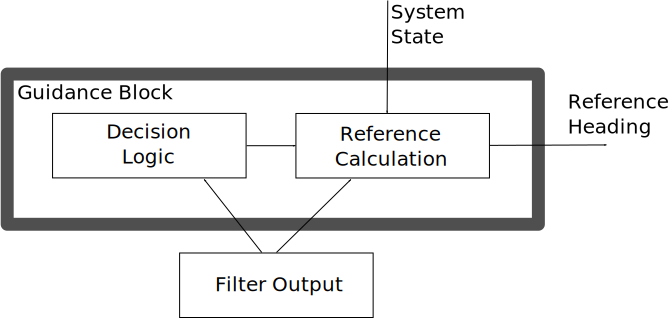
\includegraphics[width=0.8\textwidth]{pics/guidance}
		\caption{Guidance System Block}
		\label{fig:ch2-Guidance-block}
	\end{figure}

	The AUV guidance system is assumed to have three modes, \textit{searching}, \textit{tracking} and
	\textit{initialise/finalise}. The \textit{initialise/finalise}-mode is at the beginning and end of a
	mission and will not be considered in this report. 
	
	The \textit{searching}-mode is when the AUV are looking for the pipeline. When the pipeline is laid
	on the sea floor, the position may be more or less inexact, both because of sometimes the great 
	distance from the sea level to the sea bottom, and sometimes because the pipeline have ``sagged'', 
	i.e moved away from the initial position because of movement in the sea bottom caused by ocean current
	and other environmental forces. 

	\begin{figure}[htbp]
		\centering
		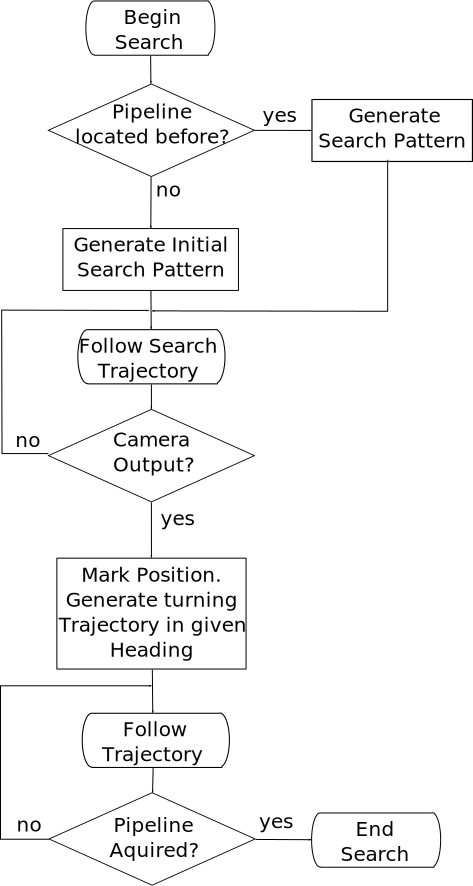
\includegraphics[width=0.5\textwidth]{pics/search_flow}
		\caption{Flow diagram of the search procedure in the \textit{searching}-mode}
		\label{fig:ch2-search-flow}
	\end{figure}
	Figure~\ref{fig:ch2-search-flow} shows the flow diagram of the searching mode. The system distinguishes 
	between two cases; the cases when the pipeline have been located before, and when it is to be found for
	the first time. If the pipeline have not been located before, the system generates a initial
	search pattern, which should be designed to cover larger area in all directions. If on the other hand the
	pipeline have been located before, another pattern should be generated, which searches the area in the direction
	the pipeline were last known to go. The
	system then follows this search pattern until it gets output from the camera, or other possible
	sensors. Then the position are marked and a turning trajectory are generated. When the pipeline
	is reacquired the guidance system goes to the tracking mode.
	\begin{figure}[htbp]
		\centering
		\includegraphics[width=0.4\textwidth]{pics/contact_trajectory}
		\caption{A turning trajectory for one possible contract}
		\label{fig:ch2-turning-trajectory}
	\end{figure}
	
	When in the \textit{tracking}-mode the AUV tries to follow the pipeline as closely as possible, and
	keep the pipeline inside the field of view as best as possible.

	\subsection{Reference Calculation}
		A look-ahead based guidance algorithm is chosen for it's simplicity and robustness. All
		together a pipeline are made up of mostly linear segments or at least almost linear
		segment. One can then assume that the direction of the pipeline can be known exact.
		No sudden turns are assumed and pipeline junctions are assumed to be non-existing. This gives
		the following equations for the reference heading:
		\begin{align}
			\psi_d &= \alpha_k + \psi_r \\
			\psi_r &= \tan^{-1} \left( \frac{-e}{\Delta} \right)\\
			e &= -(n(t) - p_x)\sin\alpha_k + (e(t) - p_y) \cos\alpha_k
		\end{align}
		
		In the presence of ocean current it will cause the heading to ``lean'' towards the current, if
		the look-ahead distance is not chosen too big. The ``leaning'' are because the current will try to
		push the AUV off the pipeline and the guidance will compensate for this. At last some kind of
		equilibrium between the current and the AUV heading will be reached. This will will work well under the
		assumption that	the current are constant.
		
	
	\subsection{Search Patterns}
		\label{subsec:ch2_searchpattern}
		It is obvious that some kind of search pattern must be implemented for this kind of
		application. This might be customised for every mission or it might be selected from a library
		of suiting search patterns. 
		This section will look at some search patterns which might be suiting for the pipeline search
		application.

		\begin{figure}[htbp]
			\centering
			\subfigure[Divergent Zig-Zag pattern for lost pipeline during tracking]{
				\label{fig:ch2_zig_zag}
				\includegraphics[width=0.4\textwidth]{pics/divergent_zig-zag}} \quad
			\subfigure[Outwards spiral pattern for initial pipeline search]{
				\label{fig:ch2_spiral}
				\includegraphics[width=0.4\textwidth]{pics/spiral_search}}
			\caption{Differnet search pattern}
			\label{fig:ch2_searchpattern}
		\end{figure}
		The first case is when the pipeline are not in its predetermined position or the position
		sensors gives out erroneous readings, some kind of search need to be initiated to find the
		pipeline. This could be something like the depicted case in Figure~\ref{fig:ch2_spiral}.
		Spiral pattern going outwards to try to find the pipeline in the vicinity of the AUV position. This
		will make the AUV cover large a large area around where the pipeline are supposed to be.
		This should be aided with other sensors, for example with a Sidescan Sonar, which provides
		sensor data in the horizontal plane around the AUV.

		The other case, is when the pipeline is lost during tracking. Since the general direction of
		the pipeline are assumed known, a divergent zig-zag pattern around the pipeline direction, from the
 		last known direction, might be a suiting pattern. This will make the AUV cover the area
		where the pipeline are assumed to go.

	
\section{Overall System}
	The system flow are depicted in Figure~\ref{fig:ch2-flowdiagram}. This is how the overall system behaves
	during a pipeline inspection mission. 
	\begin{figure}[htbp]
		\centering
		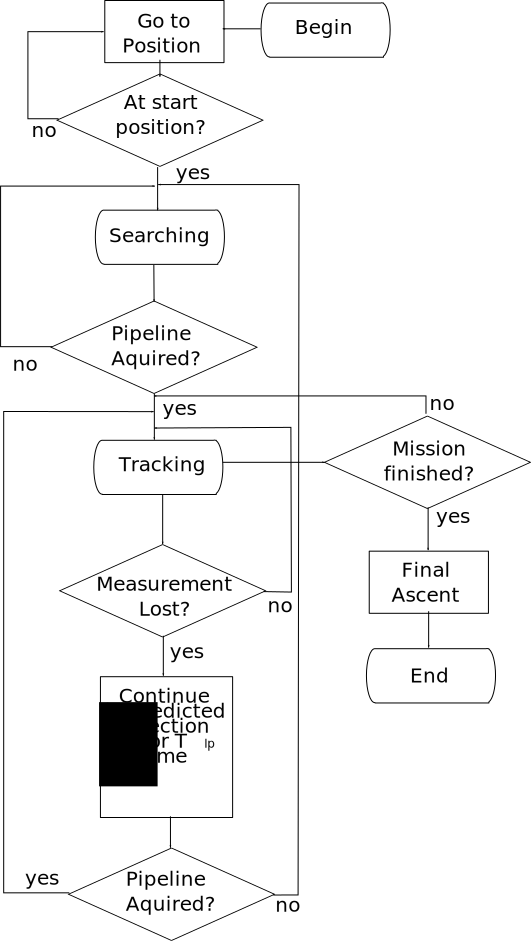
\includegraphics[width=0.5\textwidth]{pics/Operation}
		\caption{Flow diagram of pipeline inspection mission}
		\label{fig:ch2-flowdiagram}
	\end{figure}
	The system will start by moving to the point where the inspection should start. Then the searching
	procedure will be initiated if the AUV does not make contact with the pipeline immediately. It will
	search for the pipeline until it has located it, and then continue tracking until the the goal are met
	or the on-board energy storage becomes depleted. 

	There are a number of design parameters needed to be set. These parameters might be constant or
	changing between missions. They are summarised in Table~\ref{tab:ch2-design-param}
	\begin{table}[htbp]
		\centering
		\begin{tabular}{| c | p{6cm} |}
			\hline
			Design Parameter 	& 	Description \\
			\hline
			\hline
			$T_{lp}$ 		&	The Dead Reckoning time. Time before pipeline are
							considered lost. \\
			\hline
			$\Delta$		&	The lookahead distance, deciding the convergence of
							the heading to the path \\
			\hline
			$P_w$			& 	The predicted path of the pipeline in world
							coordinates or a parametrisation of it \\
			\hline
			$\mathbf{T}$		&	The values of this matrix must be chosen in accordance
							with the uncertainty of the predicted pipeline path.
							Usually chosen large \\
			\hline
			$\mathbf{Q}$ \& $\mathbf{W}$ & 	The covariance matrices of the filter, which specifies how much
							one wants to trust the predicted values of the pipeline and the
							uncertainty of the measured ones. Typically the measurements 
							should be values more than the predicted values\\
			\hline
		\end{tabular}
		\caption{Summary of design parameters in the system}
		\label{tab:ch2-design-param}
	\end{table}
	These parameters should be chosen in accordance with what kind of environmental forces there are in
	the area. Also the search patterns should be customised for every mission. To set how much area the search
	patterns need to cover, and vary the spreading angle of the divergent zig-zag pattern in accordance with how
	certain the estimate of the direction of the pipeline is.
	

